\section{Aufbau}
In Abbildung \ref{fig:Aufbau} ist der Aufbau des Versuches schematisch abgebildet.
Zur Erzeugung von Spektrallinien wird eine Cadmium-Lampe in einen Elektromagneten gebracht.
Das transversal abgestrahlte Licht der Lampe wird duch eine Objektivlinse und eine Kondensorlinse auf einen Spalt kollimiert und hinter dem Spalt durch eine Linse auf einen Geradsichtprisma fokussiert.
Hinter dem Prisma wird ein Polarisationsfilter zur Selektion der $\pi$ und $\sigma$ Linien und eine weitere Linse aufgebaut.
Da hinter diesen nun die einzelnen Spektrallinien zu sehen sind, kann eine dieser Linien durch einen weiteren, verschiebbaren Spalt ausgewählt werden.
Hinter dem Spalt wird die ausgewählte Spektrallinie durch eine Linse auf die Eintrittsfläche einer Lummer-Gehrcke Platte fokussiert.
Das hinter der Lummer-Gehrcke Platte erzeugte Interferenzmuster kann dann mit einer Digitalkamera aufgenommen und analysiert werden.

\begin{figure}[H]
  \centering
  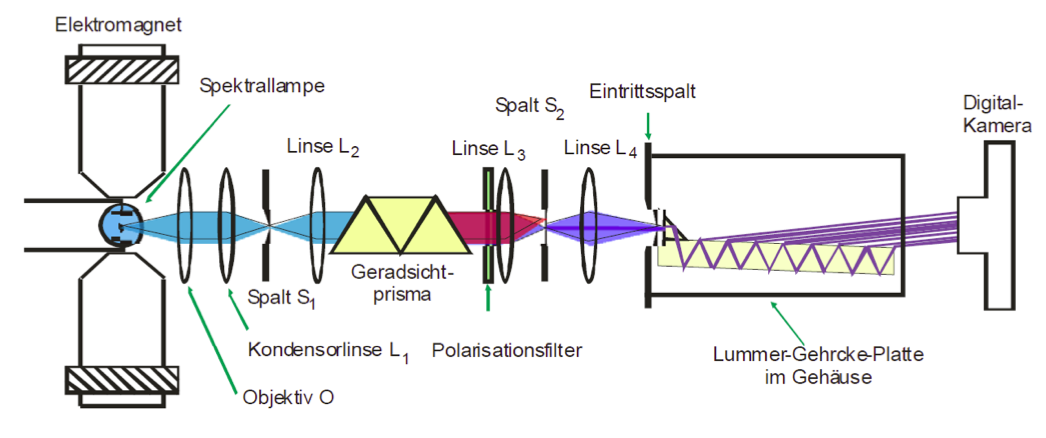
\includegraphics[width = .7\textwidth]{images/Aufbau.png}
  \caption{Schematische Darstellung des Versuchsaufbaus \cite{anleitung}.}
  \label{fig:Aufbau}
\end{figure}

\subsection{Lummer-Gehrcke Platte}

Eine Lummer-Gehrcke Platte funktioniert wie ein hochauflösendes Spektrometer mit einem sehr kleinen Auflösungsbereich.
Diese besteht aus einer planparallelen Glasplatte, das eingestrahlte Licht wird an der Oberseite der Platte reflektiert und gebrochen.
Somit kommt es auf der Länge $L$ der Platte an vielen Stellen zu gebrochenen Lichtstrahlen, welche miteinander interferieren.
Eine Zeichnung einer Lummer-Gehrcke Platte ist in Abbildung \ref{fig:Lummer-Gehrcke} dargestellt.

\begin{figure}
  \centering
  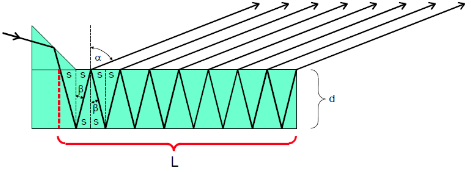
\includegraphics[width=.5\textwidth]{images/Lummer.png}
  \caption{Zeichung einer Lummer-Gehrcke Platte. An der Unterseite der Platte kommt es zur Totalreflektion, an der Oberseite tritt bei jeder Brechung ein kleiner Teil des Lichtes aus und es kommt zur Interferenz dieser austretenden Strahlen \cite{anleitung}.}
  \label{fig:Lummer-Gehrcke}
\end{figure}

Durch eine Veränderung $\delta \lambda$ der eingestrahlten Wellenlänge durch eine Veränderung des Magnetfeldes, kommt es zu Verschiebung der Interferenzstreifen.
Damit es nicht zur Überlagerung der Streifen kommt, muss das Dispersionsgebiet
\begin{equation*}
  \Delta \lambda_\text{D} = \frac{\lambda^2}{2d} \frac{1}{\sqrt{n^2-1}} \, .
\end{equation*}
der Lummer-Gehrcke Platte berücksichtigt werden.
Dieses gibt an, wie groß die Wellenlängenverschiebung maximal sein darf, sodass sich die Interferenzstreifen nicht überlagern und ist abhängig von der Dicke $d$ und dem Brechungsindex $n$ der Platte.
Um diese Grenze nicht zu überschreiten, muss das Magnetfeld in Abgängigkeit der Energieaufspaltung und damit der Landé-Faktoren $g_J$ eingestellt werden.
Für die maximale Magnetfeldstärke folgt
\begin{equation} \label{eqn:B}
  B = \frac{\Delta \lambda_\text{D}}{4} \frac{h c}{\lambda} \frac{1}{\mu_B g_J} \,.
\end{equation}
Die Magnetfeldstärke muss also vor Versuchdurchführung für die vermuteten Landé-Faktoren eingestellt werden.

\par\medskip

Die Wellenlängenverschiebung $\delta \lambda$ kann aus der Aufspaltung der Spektrallinien mit

\begin{equation}\label{eqn:WV}
  \delta s = \frac{1}{2} \frac{\delta s}{\Delta s} \Delta \lambda_\text{D}
\end{equation}

berechnet werden.
Dabei beschreibt $\Delta s$ den Abstand der Spektrallinien bei ausgeschaltetem Magnetfeld und $\delta s$ den Abstand der Spektrallinien bei eingeschaltetem Magnetfeld.
